%mainfile: ../master.tex
\chapter{Specification}

This chapter is documentation of the requirement engineering process, as describe in \cite{sommerville}. The structure will follow the elicitation process of requirements, by the methods included in sommerville's book. Some contributing methods used to describe the problem domain are borrowed from \cref{OOAD}. 

From the system definition and "rich picture" of the problem domain that the system will be operating, we can extract some classes, \quote{A description of a collection of objects with the same structure, behaviour and attributes}, as described in \cref{OOAD}. This classes will be beneficial when figuring out what we need to keep track of in the problem domain, or what is relevant in our model of the problem domain.

Classes:
\begin{itemize}
\item Person - The user of the system
\item Action - An action the system should recognise as feedback
\item Pattern - The usage patter of a user, what is typical behaviour
\item Mistake - System did something wrong by the user
\item Sensor - The observational member of the system
\item Switch - A feedback source
\item Lamp - The light source on which system action
\item Light intensity - Luminance
\item Room - What room is the user in
\item Premise - The user home enviroment
\item Time - At what time, a pattern property
\end{itemize}


%mainfile: ../master.tex
\section{Events}\label{sec:events}

\citet{OOAD} describes an event the following way: \enquote{An instantanious event that involves one or more objects}. By understanding which events can happen in the problem domain, the behaviour of objects in the problem domain can be understood, further understanding possible usecases of the system.

The events in \cref{tab:eventtable}, only showcases some possible events, that can take place in the problem domain. There are however infinitely many events that can happen, as an event can be identified as observable changes of sensor values. When choosing the events, the focus was on the events being representative of all possible events.

\begin{table}
  \centering
  \begin{tabular}{*{7}{|l}|}
    \hline
    Event & Person & Action & State & Pattern & Location & Time \\
    \hline
    Enter/leave room & \checkmark & \checkmark & \checkmark & \checkmark & \checkmark & \checkmark\\
    \hline
    Turn on/off appliance & \checkmark & \checkmark & \checkmark & \checkmark & & \checkmark\\
    \hline
    Changes in external light & & & \checkmark & \checkmark & & \checkmark\\
    \hline
    Watching TV & \checkmark & \checkmark & & \checkmark & & \checkmark\\
    \hline
    Unexpectedly late & \checkmark & \checkmark & \checkmark & & \checkmark & \checkmark\\
    \hline
  \end{tabular}
  \caption{Event table}
  \label{tab:eventtable} \kanote{Hændelserne i tabellen skal forklares, så læseren ved hvad fx. "Unexpectedly late" betyder}
\end{table}
% \begin{table}[h!]
%   \centering
%   \begin{adjustbox}{max width=\textwidth}
%     \begin{tabular}{*{8}{|l}|}
%         \hline
%         \textbf{Event}                     & Person & Action & State & Pattern & Sensor & Actuator & Location & Time   \\
%         \hline
%         User entered lo0cation (unexpected) & \cmark & \cmark & \cmark  & \cmark   & \cmark   & \cmark & \cmark   & \cmark   & \cmark \\
%         \hline
%         User entered location (expected)   & \cmark & \cmark & \cmark  & \cmark   & \cmark   & \cmark & \cmark   & \cmark   & \cmark \\
%         \hline
%         Left home & \cmark & \cmark & \cmark & & \cmark & & \cmark & & \cmark & \cmark & \\
%         \hline
%         Enter room & \cmark & \cmark & \cmark & & \cmark & & \cmark & \cmark & \cmark & & \\
%         \hline
%         Left room & \cmark & \cmark & \cmark & & \cmark & & \cmark & \cmark & \cmark & &\\
%         \hline
%         Flicked switch & \cmark & \cmark & \cmark & \cmark & \cmark & \cmark & \cmark & \cmark & \cmark & & \\
%         \hline
%         Outside/External light intensity down & \cmark & & & & \cmark & \cmark & \cmark & \cmark & \cmark & &\\
%         \hline
%         Outside/External light intensity up & \cmark & & & & \cmark & \cmark & \cmark & \cmark& \cmark & &\\
%         \hline
%         Person sleeping & \cmark & \cmark & \cmark & & \cmark & & \cmark & & \cmark & & \cmark\\
%         \hline
%     \end{tabular}
%   \end{adjustbox}
%   \caption{Event table}
%   \label{tab:eventtable}
% \end{table}

\sinote{Udkommenteret i Tex dokument, er et behaviour diagram. Hvad skal det bruges til?}
% \begin{figure}
%    \centering
%    \begin{adjustbox}{max width=\textwidth}
%     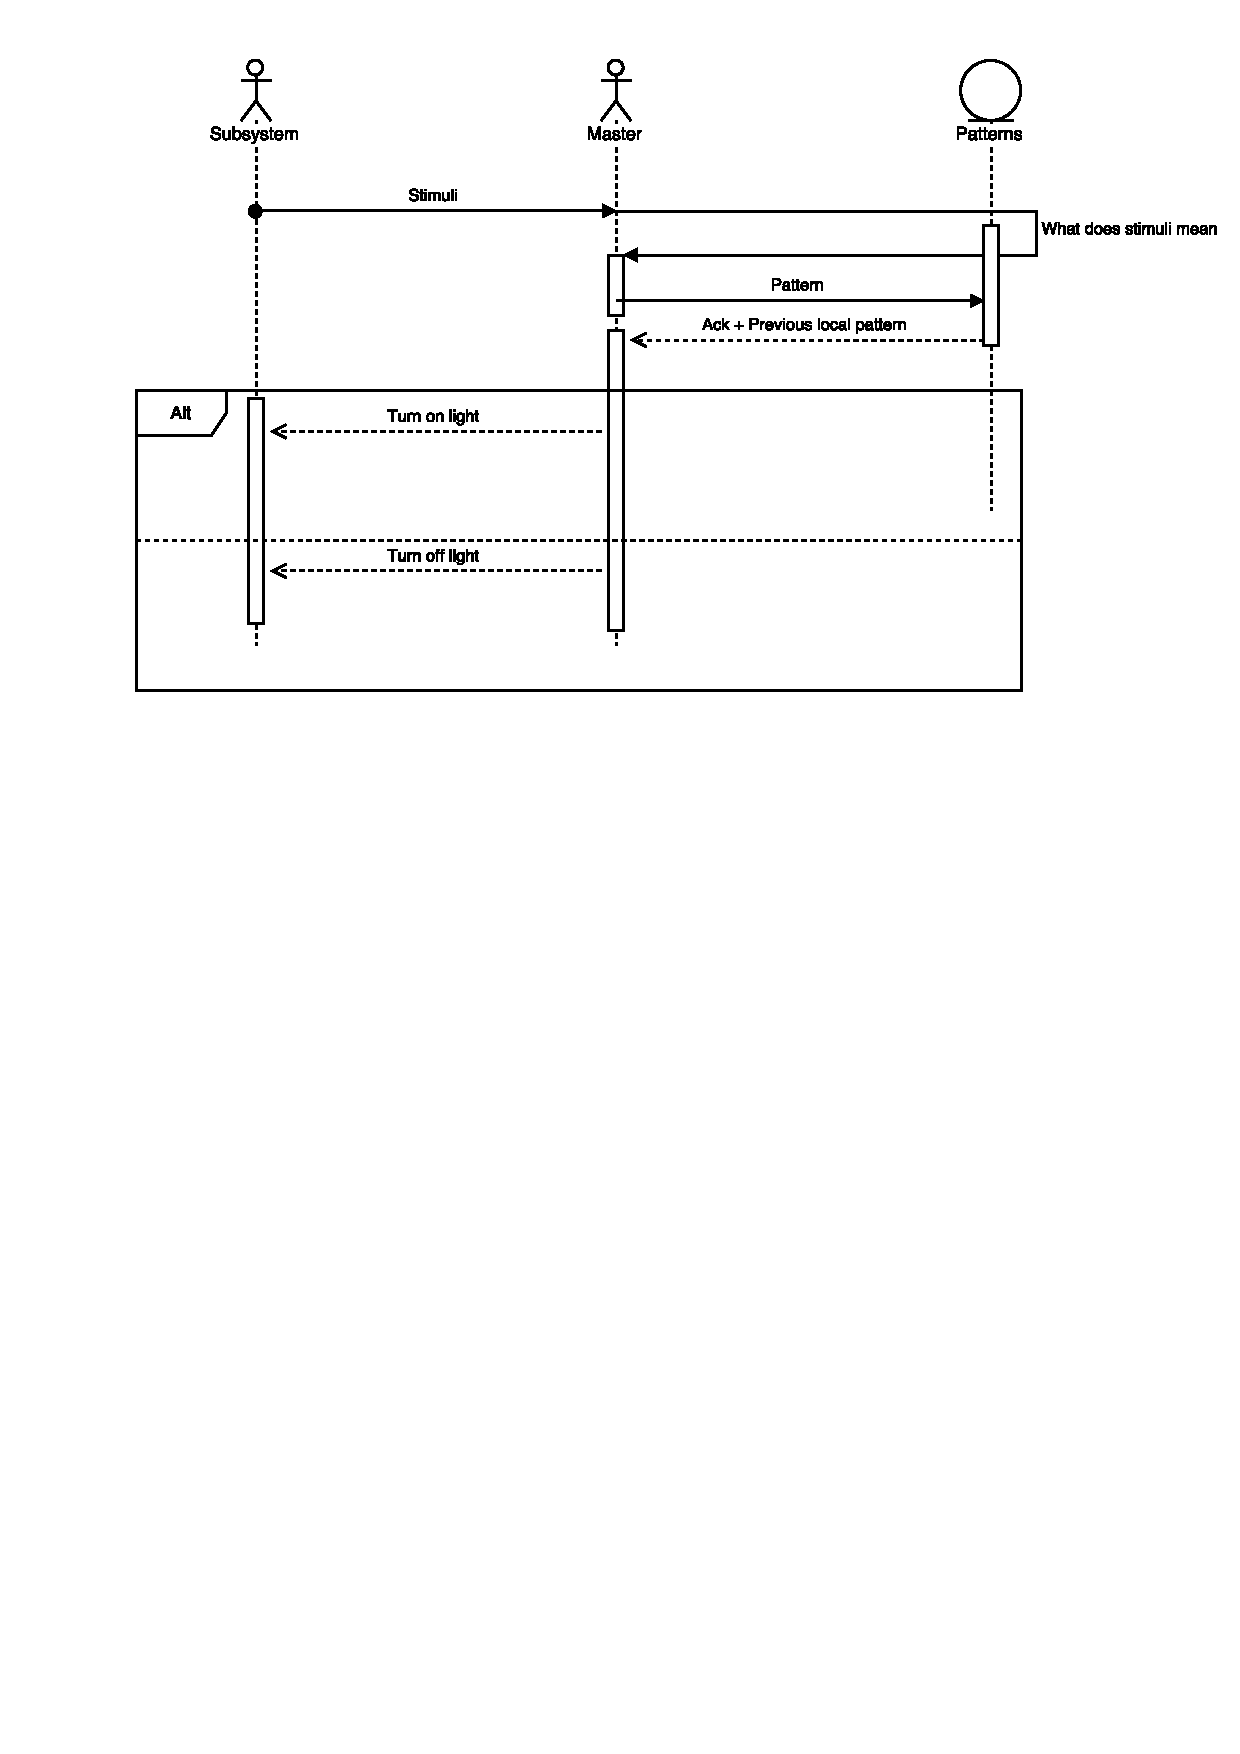
\includegraphics{Behaviour.pdf}
%    \end{adjustbox}
%    \caption{Behaviour diagram}
% \end{figure}


%mainfile: ../master.tex
\section{User scenarios}\label{sec:userscenarious}

This section will describe branches of possible narratives derived from the use cases, described in the \cref{sec:usecases}.

\textit{A user is reading a book, the light intensity of the sun is low now due the time of the day, and the user is having trouble reading. The system has learned that at this light intensity when the user is situated at the couch with tv not running, the user now wants the light to be on.}

\textit{A user is home alone in his/her living room. Now leaving a room to go the toilet but does not turn of the light in the living room, while on the toilet the user closes the door and does not observe the light in the living room being turned off by the system to conserve/save energy.}

\textit{A user just left home for a vacation, the user is leaves a few lights on due to stress, the system recognises this and switches the lights off. The user has not been home for 24 hours, the system now initiates in doing short cycles of simulating normal behaviour of the user in some rooms to seed the impression of someone being home, to proactively prevent attracting interest from any observing burglars.}

\textit{In a financial report an organisation recognises a substantial amount of funds is used on lighting the facility. The system generates a report on the lights around the facility, effective lighting hours. Which the supervisors can conclude on to argue were to invest on more energy efficient lighting. Further the system reports on broken or not functioning lighting.}


%Just for fun ? Many users is situated in the living room and the volume(db) of the stereo is really high, so users is shouting to hear each other and this occurs over prolonged duration, the system intellingently lowers the volume without the user noticing. And at 1am/pm(night) the user normally goes to sleep but not today, but because of neighbors the system lowers the volume further.



%mainfile: ../master.tex
\section{Use cases}\label{sec:usecases}

This section will describe ways of interacting with the prototypical system derived from the requirements.

<<<<<<< HEAD
<<<<<<< HEAD
<<<<<<< HEAD
=======
>>>>>>> 9c8f5030b9365c258596d255a2898784b52995cb
\begin{figure}
 \centering 
 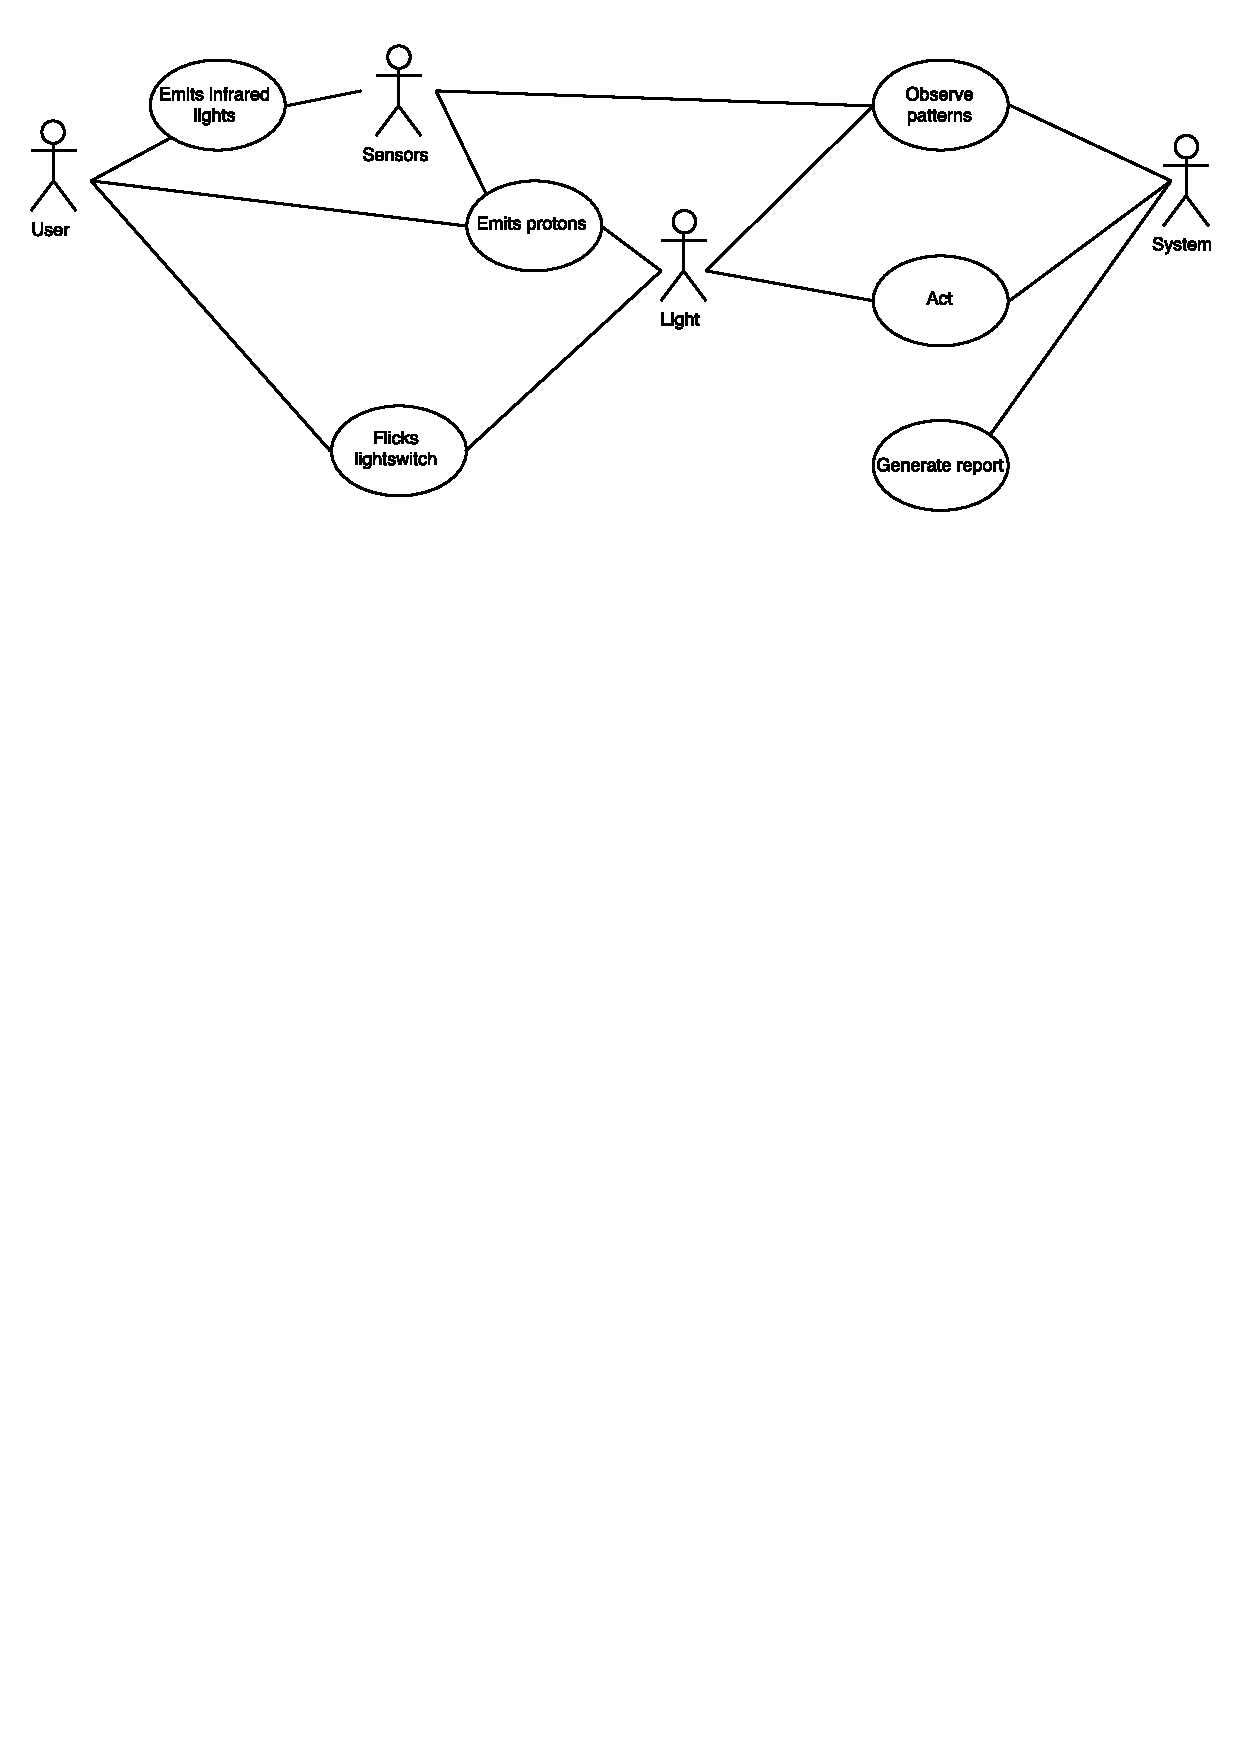
\includegraphics{Usecases.pdf}
 \caption{Rich picture of the problem domain}
\end{figure}
<<<<<<< HEAD
=======

>>>>>>> Specification refactor
=======
\begin{figure}
 \centering 
 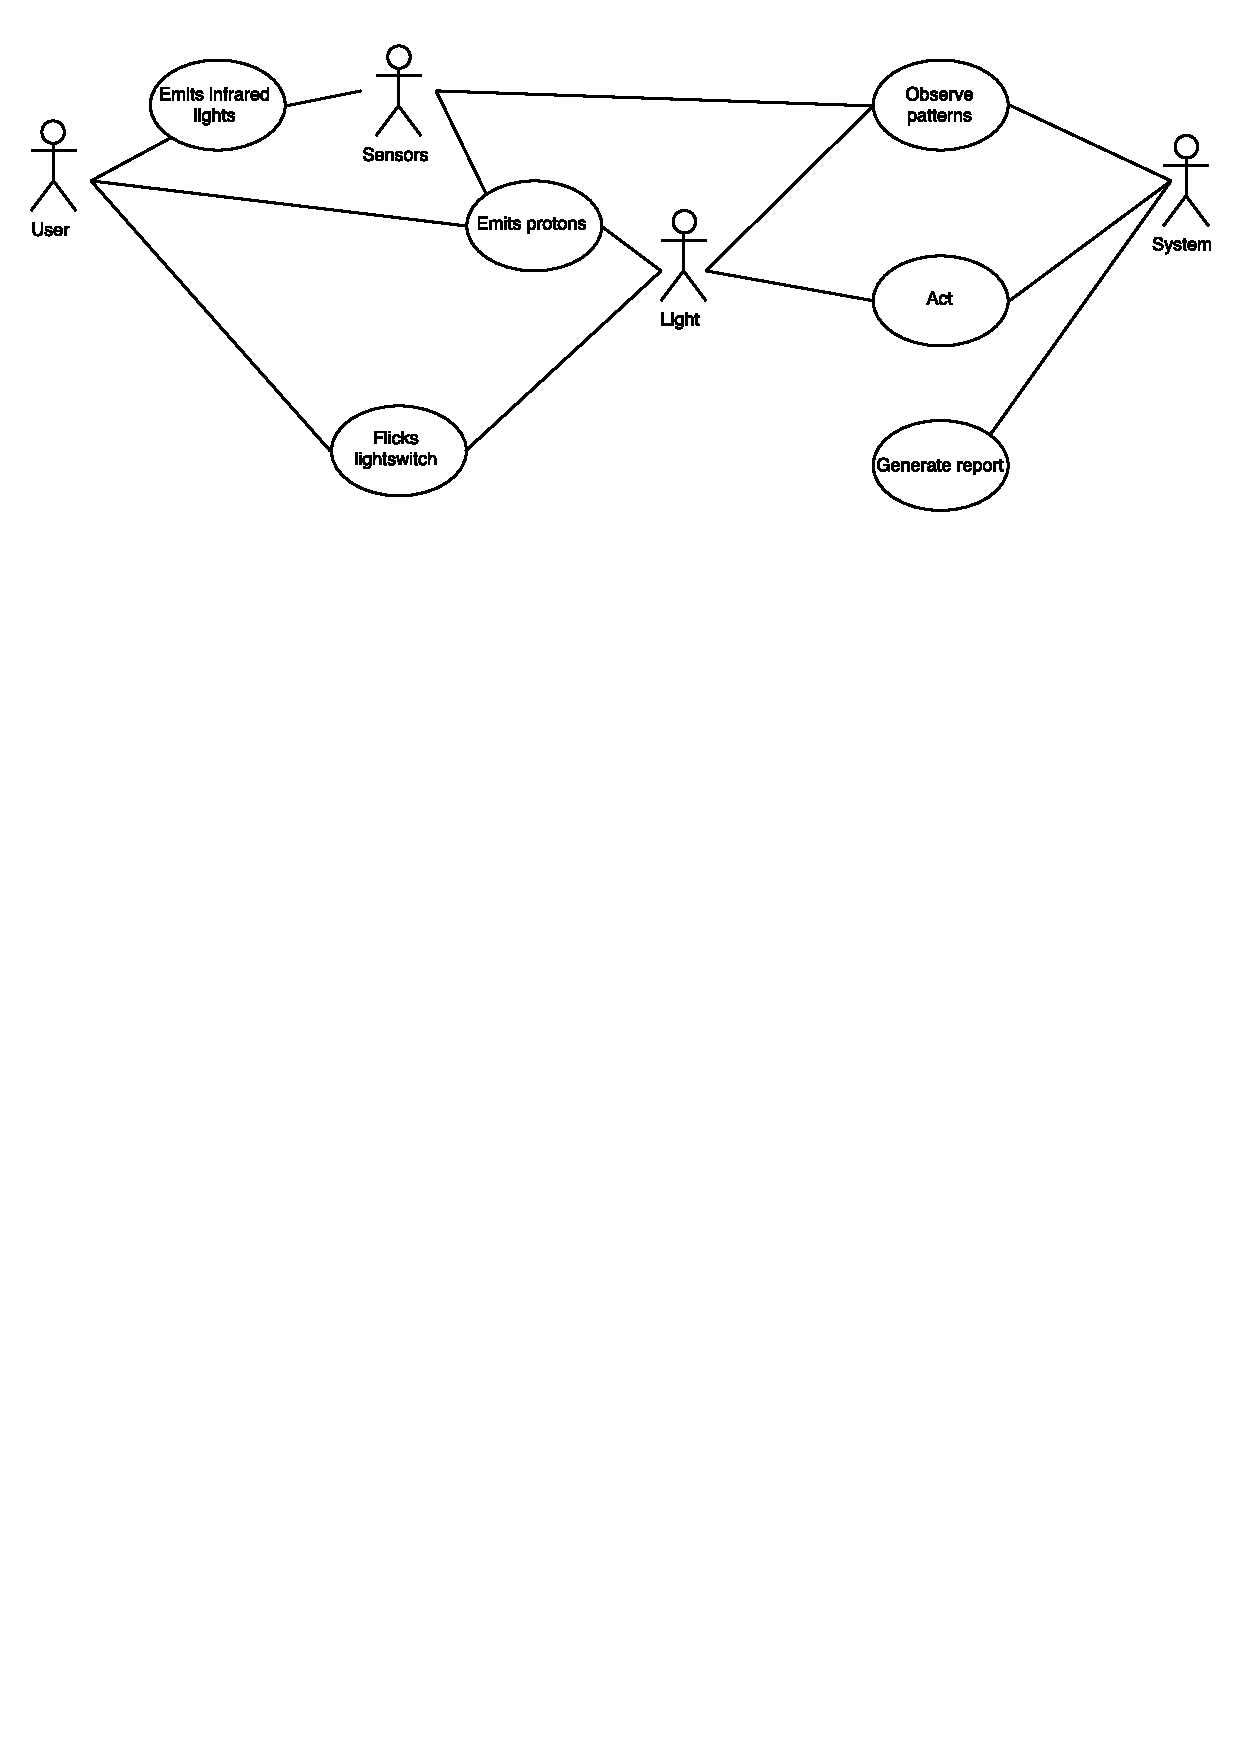
\includegraphics{Usecases.pdf}
\end{figure}
>>>>>>> More user scenarios
=======
>>>>>>> 9c8f5030b9365c258596d255a2898784b52995cb


%mainfile: ../master.tex
\section{structure}\label{sec:structure}

This section will describe what classes are associated to what classes. This will be useful for the designers and system when designing and reasoning about the knowledge base \cref{sec:KB}.





Elicited requirements: %Mangler argumentation

\begin{itemize}
\item The light in a users home will be turned off only when there is no need for it.
\item The user should be in doubt that the system will eventually turn off the light.
\item The should not be afraid that the system will suddenly turn off the light, whilst the user is need of it.
\item The light management should sought to be invisible to the user, light is turned on before a user can observe this behaviour.
\item Will learn usage patterns of the user, turn on light at specific time of day or at a specific light intensity.
\end{itemize}
